
\chapter{Introduction} \label{Introduction}
This thesis discusses the bachelor project `Satogaeri' for the computational logic research group at the University of Innsbruck. The project was proposed as part of the logic puzzle focus\footnote{http://cl-informatik.uibk.ac.at/software/puzzles/} of the mentioned research group. Over the years several solvers for Japanese puzzles similar to Sudoku have been developed to demonstrate how logic can be used in problem domains known by a broad audience.

The project had the following aims: 
\begin{enumerate}
	\item implement a solver for Satogaeri puzzles,
	\item implement a generator for Satogaeri puzzles,
	\item implement a tool that has (at least) the same functionality as the Satogaeri player of Nikoli\footnote{http://www.nikoli.com/en/puzzles/satogaeri/} and incorporates (1) and (2).
\end{enumerate}

While reading this thesis one will be lead through the steps how those aims were met and additionally will be given some further background information concerning Satisfiability Modulo Theories (Section~\ref{Satisfiability Modulo Theories}) and JavaFX (Section~\ref{JavaFX}).

However everything can be improved therefore some thoughts about future optimisations and work are added in the Conclusion (Section~\ref{Conclusion}).

Furthermore there was an optional task to prove that the Satogaeri puzzle problem is an NP-complete problem. Unfortunately this point was not fulfilled during the project.

\chapter{Satogaeri} \label{Satogaeri}
Satogaeri is a logic puzzle published by the Japanese company Nikoli Ltd. in 2002. Satogaeri only made a booklet appearance in Nikoli Vol. 99, Vol. 100 and Vol. 101. However it got revived on nikoli.com in 2013.

\section{Rules}
The official rules from Nikoi state:

\begin{enumerate}
  \item The areas enclosed by bold lines, are called ``Countries". Move the circles, vertically or horizontally, so each country contains only one circle.
  \item The numbers in the circles indicate how many cells they have to pass through. Circles without numbers may move any distance, but some of them do not move.
  \item The circles cannot cross the tracks of other circles and cannot go over other circles. 
\end{enumerate}
And additionally the 4th rule, which counts for every logic puzzle:
\begin{enumerate}
  \item[4] A puzzle only has one solution.
\end{enumerate}

\begin{figure}
  \centering
  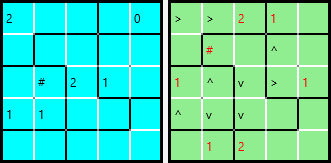
\includegraphics[width=0.9\textwidth]{Pictures/sample_small.png} 
  \caption{Small sample puzzle with its solution}
  \label{fig:sample_small}
\end{figure}

Handcrafted puzzles tend to have a mirrored country-layout either vertically, horizontally or both as can be seen in Figure~\ref{fig:sample_small}.

\chapter{Satisfiability Modulo Theories} \label{Satisfiability Modulo Theories}
Before we can go on and talk about how to solve Satogaeri problems we first have to look into Satisfiability Modulo Theories (SMT) for this was used to create the solver and the generator.

SMT can be seen as an enhancement of traditional Satisfiability (SAT) solving. In SAT solving one tries to find an interpretation of a given problem, where this interpretation is a boolean formula composed of boolean variables and expressions like AND, OR and NOT; to state a few. If this constructed formula has a configuration of its variables where the formula evaluates to `true', then also the original problem must have a solution. A satisfying configuration of the variables often gives a good clue on how to solve the original problem.

To state an example: the formula
\[(a \lor b \lor (\neg c)) \iff ((\neg a) \land c)\]
is satisfied with the assignment \textit{a} is 'false', \textit{b} and \textit{c} are 'true'. Therefore the problem interpreted by this formula must be solvable too.

SMT goes one step beyond that by replacing some boolean variables with predicates. A predicate is basically a binary-valued function of non-binary variables, which allows us to have function symbols with different arities. Now we can express formulas in first-order logic like
\[x > y \land 3 x + 4 \leq 4 y\]
where a natural number can be seen as a function symbol with arity 0, a so called constant.
There are many different approaches of implementing SMT solvers, but the two major ones are the \textit{eager} and the \textit{lazy} approach.

\section{Eager SMT}
In the \textit{eager} approach one tries to convert the given formula into an equisatisfiable propositional formula with all the additional needed constraints of the originating problem. With these constraints the search-space should be reduced so that a common SAT solver can solve the formula much quicker. And this is the appealing part of this approach: one can use already existing SAT solver to finally check the satisfiability. However the converting process into a propositional formula can be cost-intensive.\cite{2009satisfiability}

\section{Lazy SMT}
The \textit{lazy} approach consists of two parts. The first part are theory-specific solvers ($\mathcal{T}$-solvers) to handle conjunctions of literals, which are embedded again into a SAT solver. The advantage of incorporating $\mathcal{T}$-solvers is that one can use a specific algorithm and data-structure which fits the problem at hand best. This should lead to a better performance.\cite{sebastiani2007lazy}

\section{SMT-Library}
The SMT library (SMT-Lib) was found in 2003 to provide common standards and a library of benchmarks for diverse SMT solvers. With this standards and benchmarks evaluation and comparison of SMT systems should be made easier to give the research a competitive touch, which ultimately should result in advancing the state of the art in SMT. They even organize an annually SMT solver competition (SMT-COMP).

SMT-Lib was greatly useful for this thesis by providing an easily understandable syntax which made many SMT-Solver accessible, like Boolector, CVC4 and MathSAT 5 to name a few. On their web-site\footnote{www.SMT-LIB.org} one can find a long list of solvers supporting SMT-LIB and a separate list of these solvers still under active development.

\section{Logics}
SMT-LIB supports a huge variety of different logics. The advantage here is to be able to apply more specialized and therefore more efficient algorithms.
\begin{figure}
  \centering
  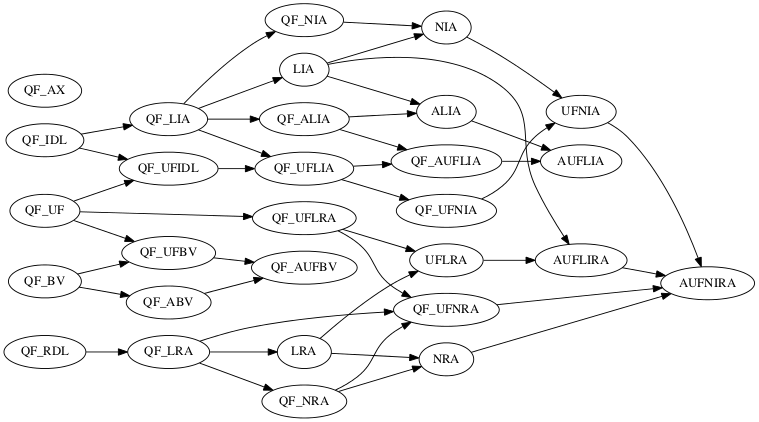
\includegraphics[width=0.9\textwidth]{Pictures/logics.png}  
  \caption{A link from a logic L1 to a logic L2 means that every formula of L1 is also a formula of L2}
  \label{fig:logics}
\end{figure}
The meaning of the logics in Figure~\ref{fig:logics} is letter coded. For example:
\begin{enumerate}
  \item QF stands for the restriction to quantifier free formulas
  \item IA stands for the theory Ints (Integer Arithmetic)
  \item L before IA, RA, or IRA stands for the linear fragment of those arithmetics 
\end{enumerate}
So QF\_LIA is an unquantified linear integer arithmetic. In essence, Boolean combinations of inequations between linear polynomials over integer variables. Beside this logic we will also use the QF\_UF logic throughout this project. QF\_UF is the logic of Quantifier-Free Uninterpreted Functions. It incorporates just the Core theory, providing the Bool sort and the various standard operations on Boolean values.
 
The whole explanation can be found on the SMT-Lib web-site\footnote{www.SMT-LIB.org} in the section Logics.

\section{CVC4}
The SMT-Solver used in this project is the Cooperating Validity Checker 4 (CVC4), currently the most novel  successor of the Stanford Validity Checker which was found in 1996. CVC4 is a joined project of the New York University and the University of Iowa.

Supported features are including: several built-in base theories, support of quantifiers and a model generation ability. The latter is a very important requirement for this project at hand.

Furthermore CVC4 has its own wiki\footnote{http://cvc4.cs.nyu.edu/wiki} with useful tutorials, a user manual and a developer section.

\chapter{Solver} \label{The Solver}
Now we will discuss how to represent a Satogaeri puzzle in SMT and what are the required inputs for the CVC4 solver. Because we use the SMT-Lib and its generalized input syntax the CVC4 solver could be replaced by any other solver supporting the SMT-Lib. For illustration purposes we will now manually create a SMT representation of the Satogaeri puzzle of Figure~\ref{fig:solver_example}.
\begin{figure}
  \centering
  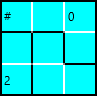
\includegraphics[scale=1]{Pictures/Solver_example.png} 
  \caption{Trivial Satogaeri puzzle}
  \label{fig:solver_example}
\end{figure}

\section{Presetting}
Before starting up the CVC4 solver we need to ensure some presetting which is mandatory for our purpose.
The parameter additionally given to the program via the command-line are the following:
\begin{lstlisting}
--lang smt -m --statistics
\end{lstlisting}

\emph{--lang smt} enables the use of the SMT-Lib syntax other than the regular CVC4 syntax.

\emph{-m} enables the generation of a model which means once our problem is satisfiable the solver also generates a satisfying assignment for all variables to give us an example model in which the problem has a solution.

\emph{--statistics} prints a long list of statistics if our problem was satisfiable. We will use these statistics to decide how `difficult' the given Satogaeri puzzle was. More about that later in Section~\ref{Statistics}. 

\section{Declaring Functions}
Now that CVC4 is started with the proper presetting we can start our representation of the puzzle in Figure~\ref{fig:solver_example}.

The first thing to do is to define the logic to be used:
\begin{lstlisting}
(set-logic QF_LIA)
\end{lstlisting}
In our case it is the unquantified linear integer arithmetic. Simple because we do not need quantifiers nor anything other than simple integer functions. By restricting the search-space for the solver it should be faster in finding a solution.

Finally we can start our SMT-interpretation of the Satogaeri puzzle. First of all we define every cell of the puzzle as a variable integer. One can think of the puzzle as a 3-by-3 matrix filled with yet unknown numbers.
\begin{lstlisting}
(declare-fun f1-1 () Int)
(declare-fun f1-2 () Int)
(declare-fun f1-3 () Int)
(declare-fun f2-1 () Int)
(declare-fun f2-2 () Int)
(declare-fun f2-3 () Int)
(declare-fun f3-1 () Int)
(declare-fun f3-2 () Int)
(declare-fun f3-3 () Int)
\end{lstlisting}
This lines introduce a new function with the name e.g. `f2-3' which has no arguments (empty brackets) and returns an integer. `f2-3' in our case represents the field in row 2 and column 3 (top to bottom, left to right). The collection of these functions will be our matrix, to be more precise its the matrix where we will define our 'country' restrictions of the Satogaeri rules, referred to as country-matrix from here on.

Now we will create a second 3-by-3 matrix just to model the restrictions of the circles.
\begin{lstlisting}
(declare-fun c1-1 () Int)
(declare-fun c1-2 () Int)
(declare-fun c1-3 () Int)
(declare-fun c2-1 () Int)
(declare-fun c2-2 () Int)
(declare-fun c2-3 () Int)
(declare-fun c3-1 () Int)
(declare-fun c3-2 () Int)
(declare-fun c3-3 () Int)
\end{lstlisting}
Same principle as before only that the `c' in `c2-3' stands for circle.

One can think of it as a circle-matrix on top of a country-matrix and both only check for specific rules of the Satogaeri puzzle.

\section{Country Rules}
We declared a country-matrix but there are no restrictions on it whatsoever. Next we address the encoding of the rule: `one or several fields combined result in a country. Every country only can be occupied by one circle.'

For example `f1-2' and `f1-3' combined are one country. That means once `f1-2' is occupied `f1-3' is not allowed to accommodate any circles and vice versa. Later on we will define that a circle is a positive natural number, where as the absence of a circle is modelled as `0'. In the SMT syntax it will look like
\begin{lstlisting}
(assert (or (and (> f1-2 0) (= f1-3 0)) 
(and (< f1-2 0) (= f1-3 0))))
\end{lstlisting}
Important to state is that the SMT syntax consists only of prefix notations. 

\emph{assert} will make sure that in the end there is an assignment to these fields that this line will become `true' otherwise the problem is unsatisfiable. The \emph{or} states that at least one of its arguments must be `true', and the \emph{and} only yields `true' if all of its arguments evaluate to `true'. Both \emph{or} and \emph{and} can take one or more arguments inside its brackets whereas \emph{assert} only takes one.

This line basically translates to: either f1-2 is a positive number and f1-3 is zero or vice versa.

Now we have successfully translated rule number 1 into SMT-syntax for one country. Let's do the same with the other two countries:

\begin{lstlisting}
(assert (or 
(and (> f1-1 0) (= f1-2 0) (= f1-3 0) (= f2-3 0)) 
(and (= f1-1 0) (> f1-2 0) (= f1-3 0) (= f2-3 0)) 
(and (= f1-1 0) (= f1-2 0) (> f1-3 0) (= f2-3 0)) 
(and (= f1-1 0) (= f1-2 0) (= f1-3 0) (> f2-3 0))))

(assert (or (and (> f2-2 0) (= f3-2 0) (= f3-3 0)) 
(and (= f2-2 0) (> f3-2 0) (= f3-3 0)) 
(and (= f2-2 0) (= f3-2 0) (> f3-3 0))))
\end{lstlisting}
And we are done with the country-matrix.

\section{Circle Rules}
First thing we do is to assign every circle with its own ID.
\begin{lstlisting}
(assert (and (= c1-1 1) (= c1-3 2) (= c3-1 3)))
\end{lstlisting}
At the start of this section we defined c1-2 as a function with no arguments which yields an integer. All we did was to define that this integer has to be 1. In other words: c1-2 is constant 1.
Now the `empty'-circle at c1-1 has the ID 1, `0'-circle at c1-3 has the ID 2 and so on.

Our next step is to define the possible moves every circle is able to make. Let's start of with the easiest: the `0'-circle at c1-3. The 0 indicates that this circle is not allowed to move at all which means he will occupy the field he is already in.
\begin{lstlisting}
(assert (= f1-3 c1-3)))
\end{lstlisting}
We have our first interaction with the country-matrix and the circle-matrix. With this line we declare that function f1-3 has to yield the same value as c1-3 which is its ID: 2. This leads to, as we remember, that the country consisting of f1-1, f1-2, f1-2 and f2-3 is occupied and every field in this country except f1-3 has to be zero, in other words is not allowed to be occupied by any circle.

Next is the `2'-circle in c1-3. This circle can move to 2 positions either to c1-1 or c3-3 because of its movement-range of 2.
\begin{lstlisting}
(assert (or (and (= c3-2 c3-1) (= c3-3 c3-1) (= f3-3 c3-1)) 
(and (= c2-1 c3-1) (= c1-1 c3-1) (= f1-1 c3-1))))
\end{lstlisting}
In this case we not only override the position in the country-matrix but also all the fields we pass in the circle-matrix, because rule 3 states: `The circles cannot cross the tracks of other circles and cannot go over other circles.' By leaving the ID of every circle in the fields they passed we basically leave a track which is not allowed to be crossed.

For example: the `2'-circle in c1-3 is not allowed to move to c1-1 because `empty'-circle is already there. We made sure of this by first defining the constant c1-1 with the ID 1 and now we said if the `2'-circle wants to occupy f1-1 it has to leave its ID in c1-1, which yields a contradiction because a constant can never be both 1 and 3.

To make a long story short: in this case only f3-3 can be reached and occupied without violating any rules.

Last one is the `empty'-circle at c1-1. Because of rule 2: `Circles without numbers may move any distance, but some of them do not move.' this circle has 5 possible moves to make. Either stay at c1-1, move to c1-2, move to c1-3, move to c2-1 or move to c3-1. 

It is worth mentioning that the final solver is smart enough to detect simple collisions like if there is a circle in the path beforehand and will not add that particular move to the SMT encoding, this reduces the possible cases the CVC4 solver has to check.

In this case moving to c1-3 and moving to c3-1 is not an option
\begin{lstlisting}
(assert (or (and (= f1-1 c1-1)) 
(and (= c1-2 c1-1) (= f1-2 c1-1))
(and (= c2-1 c1-1) (= f2-1 c1-1))))
\end{lstlisting}
Now we are done. The Satogaeri puzzle of Figure~\ref{fig:solver_example} is translated into SMT.


\section{Solution}
Once we translated the puzzle into an SMT-problem we can evoke the solving procedure by simply typing
\begin{lstlisting}
(check-sat)
\end{lstlisting}
Now there are 3 possible outputs the solver can give:
\begin{enumerate}
  \item unsat: It means that there is no possible assignment to solve the problem at hand.
  \item unknown: Is used when a solver did not manage to establish whether the set of assertions is satisfiable or not. However some solver will create a candidate model.
  \item sat: There is at least one possible assignment which satisfies the problem.
\end{enumerate}
Obviously we looking for a sat result. Once the problem is sat and we enabled \emph{-m}, the model generation, we now can check for possible assignments of all fields in the country-matrix as well as in the circle-matrix. Our major interest lies in the country-matrix:
\begin{lstlisting}
(get-value (f1-1))
(get-value (f1-2))
(get-value (f1-3))
(get-value (f2-1))
(get-value (f2-2))
(get-value (f2-3))
(get-value (f3-1))
(get-value (f3-2))
(get-value (f3-3))
\end{lstlisting}
Fields that are not occupied by any circle will yield a zero. However the occupied once will give us the ID-number of the circle which is currently occupying this field, the whole country.

We could also look into the circle-matrix with these lines:
\begin{lstlisting}
(get-value (c1-1))
...
(get-value (c3-3))
\end{lstlisting}
However there we will only see the path taken of every circle marked with its ID and the unneeded fields will be filled with random numbers most likely 0, but it could also be a number used as an ID for a circle which makes the circle-matrix inaccurate.

The output of the solver in this case looks like:
\begin{lstlisting}
((f1-1 0))
((f2-1 0))
((f3-1 3))
((f1-2 1))
((f2-2 0))
((f3-2 0))
((f1-3 0))
((f2-3 0))
((f3-3 2))

((c1-1 1))
((c2-1 0))
((c3-1 3))
((c1-2 1))
((c2-2 0))
((c3-2 0))
((c1-3 2))
((c2-3 2))
((c3-3 2))
\end{lstlisting}

\section{Quantifier-Free Uninterpreted Functions}
In the hope of speeding up the solving process the logic of Quantifier-Free Uninterpreted Functions was tested too. This logic provides only a few core functions but all we actually need to model a Satogaeri puzzle are equations and inequations.

Let us look into the SMT encoding of this logic. First we enable this particular logic
\begin{lstlisting}
(set-logic QF_UF)
\end{lstlisting}
 
Similar to the QF\_LIA logic we will build up 2 matrices with variables but this time Integers are not included in our repertory. So we have to introduce a new sort symbol via
\begin{lstlisting}
(declare-sort A 0)
\end{lstlisting}
This introduces a new sort called A which takes 0 parameters. The next step is to define the variables of this sort A.
\begin{lstlisting}
(declare-fun f1-1 () A)
...
(declare-fun f3-3 () A)

(declare-fun c1-1 () A)
...
(declare-fun c3-3 () A)
\end{lstlisting}

In the QF\_LIA we would have now stated that if a field is occupied by a circle the rest of the country has to be zero. Now that we do not have any numbers we need to define a symbol that represents this zero.
\begin{lstlisting}
(declare-fun zero () A)
\end{lstlisting}
To keep a link to the previous SMT encoding we simply name this new symbol zero.

Now we model the country restriction. Last time we said: `If a field is greater than zero the rest has to be zero.' Which could also be stated as: `If a field is unequal to zero the rest has to be equal to zero."

For example:
\begin{lstlisting}
((assert (or (and (distinct f2-1 zero) (= f3-1 zero)) 
(and (= f2-1 zero) (distinct f3-1 zero)))))
\end{lstlisting}

Our next step will be to distinguish all circles and zero from each other. Last time we did that via IDs but this time we simply use distinct:
\begin{lstlisting}
(assert (distinct c1-1 c1-3 c3-1 zero))
\end{lstlisting}

All that is left is the circle trace rule which is encoded exactly like what we did with the QF\_LIA logic. We use the `empty'-circle as an example:
\begin{lstlisting}
(assert (or (= f1-1 c1-1) 
(and (= c1-2 c1-1) (= f1-2 c1-1)) 
(and (= c2-1 c1-1) (= f2-1 c1-1))))
\end{lstlisting}

The \emph{(check-sat)} and the \emph{(get-value ())} command work exactly like before. To see the full encoding in QF\_UF and the corresponding output please go to the Appendix section.

To see how the QF\_UF encoding held up against the QF\_LIA encoding time-wise please got to Section~\ref{Statistics}.

\chapter{Generator} \label{The Generator}
\begin{figure}
  \centering
  \includegraphics[scale=1]{Pictures/generator.png} 
  \caption{Generator graphical interface}
  \label{fig:generator}
\end{figure}
The Generator should be able to generate random Satogaeri puzzles with varying size and difficulty. The user enters the width and height of the desired puzzle and another parameter called Countrysize which is a rational number between 0.0 and 1.0. (Figure~\ref{fig:generator}) The higher the value of Countrysize the more likely it is to get larger countries. The idea was that the more smaller countries are generated the more difficult the puzzle may get. Unfortunately it contributes very little to the difficulty of the generated puzzle.

\section{Country Generation}
As mentioned before the user defines the width and height of the puzzle. Now the program will take the topmost leftmost field which is not yet involved in any country and will declare it as a new country. With the probability of \emph{Countrysize} each of the four connecting fields (top, bottom, left, right) will be added to this newly created country. Next the four connecting fields of each new member have a chance of \emph{\((previous\_chance)^2\)} to be added too, until there are no new members.

Theoretically with this algorithm it is possible to generate countries in every conceivable shape, however some general shapes are more likely than others. And a very small Countrysize-value will end up in puzzles with a lot of countries consisting only of one field which are too easy.

\section{Circle Generation}
After we know the layout of all the countries we can start adding Circles. The Generator now randomly picks one field in every country and declares it as the home field of the circle. At this point we do have the solution to the upcoming puzzle. The next step is to shuffle these circles around.

Therefore the Generator randomly picks a direction in which the circle should move and calculates the distance to the next obstacle (e.g.: the boarder of the puzzle, another circle, the track of another circle). Another random number will be picked between 1 and the distance to the next obstacle and this indicates the movement of this circle. 

However if the obstacle is right next to the circle a new direction will be chose. If that scenario happens twice in a row, it will become a `0'-circle. This is necessary to reduce the number of boring `0'-circles but do not remove them in general.

Now everything is generated except `empty'-circles. Those are not be picked randomly but must meet some requirements. A circle will become a `empty'-circle if and only if:
\begin{enumerate}
  \item from its home filed on into the moving direction it has to leave its country with the first field
  \item in the opposite direction on the origin point there must be a blockade (a circle-trace, a circle, a border or a different country)
  \item if it is a `0'-circle it should not be possible to reach another field inside the own country
\end{enumerate}
If one of these requirements is violated it will break the uniqueness of the puzzle.

\section{Verifying Uniqueness}
Uniqueness of the solution to a puzzle is very important for the joy of play. In other words the Generator must assure that the puzzle only has one solution. This is done by simply giving the puzzle to the solver with an additional constrain which negates the solution, and if the solver finds a different solution the uniqueness of the puzzle is violated.

But how to model this additional constrain in SMT? To answer that we will look again at the puzzle in Figure~\ref{fig:solver_example}. But this time we need the solution to this puzzle which looks like in Figure~\ref{fig:solver_example_solution}.
\begin{figure}
  \centering
  \includegraphics[scale=1]{Pictures/solver_example_solution.png} 
  \caption{Solution to trivial Satogaeri puzzle}
  \label{fig:solver_example_solution}
\end{figure}
We remember that for example the `empty'-circle had the ID 1 and now occupies the field in f2-1. So all we have to do is to tell the home field f2-1 of the `empty'-circle that the ID 1 is not allowed to land there. And the same goes for the rest of the circles. In the SMT syntax it will look like this:
\begin{lstlisting}
(asser (or (not (= f2-1 1)) (not (= f1-3 2)) (not (= f3-3 3))))
\end{lstlisting}
If this line is added to our previous example of SMT encoding we have the same SMT problem as before however the solution found in Figure~\ref{fig:solver_example_solution} is prohibited.

Giving this encoding to the solver will return \emph{unsat} if the given solution is the only one and will return \emph{sat} if there is a second possible solution. Because we enabled the model generating feature we can also have a look at this second solution via the \emph{(get-value ())} input.

In other words after shuffling the numbers the generator checks for a second solution other than the home field positions of the circles, if he finds a different solution he will simply re-shuffle the circles until the home field positions are the unique solution to the puzzle.

\chapter{Tool} \label{The Tool}
With the tool one should be able to play crafted and generated Satogaeri puzzles. In addition to that one has the option of drawing puzzles and save them as .pzl files. These files can of course be loaded by the tool so one can share puzzles and play puzzles created by others.

\section{Usability}
\begin{figure}
  \centering
  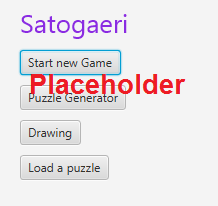
\includegraphics[scale=1]{Pictures/main_menu.png} 
  \caption{The main menu}
  \label{fig:main_menu}
\end{figure}
In Figure~\ref{fig:main_menu} we can see the main menu and its options.

\subsection{New Game} will open up another menu where on can choose a difficulty for the upcoming puzzle which ranges from Easy, Medium to Hard. After choosing the difficulty one has the option between a few puzzles which were created and published by Nikoli\footnote{http://www.nikoli.com/en/puzzles/satogaeri/}.

By dragging the numbers the player can move the circles around, however only vertical and horizontal. Once a number moved into a country this country will turn green to mark the habitation, this feature can be deactivated by the check-box \emph{colored countries}.
\begin{figure}
  \centering
  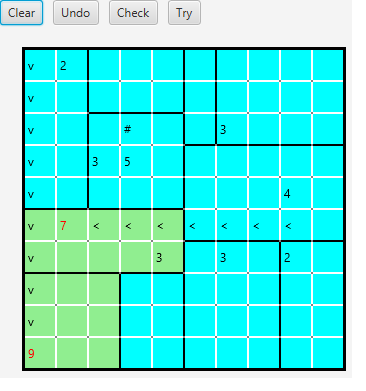
\includegraphics[scale=1]{Pictures/game.png} 
  \caption{The game itself}
  \label{fig:game}
\end{figure}
As can be seen in Figure~\ref{fig:game} the game also consists of four buttons.

\emph{Clear} returns the origin state of the game, where no circle is moved yet.

\emph{Undo} reverses the last step the user made. (up to 25 steps)

\emph{Check} checks if the puzzle is solved at the current stage.

\emph{Try} enables try mode which basically saves the current state of the puzzle. The \emph{Try} button will be replaced by \emph{Fix} and \emph{Delete} buttons. Fix will disable try mode and keeps all changes the user made during try mode. Delete will also disable try mode, however will return the old, saved state of the puzzle.

\subsection{Generator} will lead to the generator menu which was already shown and explained in Section~\ref{The Generator}.

\subsection{Drawing} leads to similar menu like in Generator where one can choose the width and height of the puzzle and this is followed by a screen similar to the one in Figure~\ref{fig:drawing_screen}.
Now one can draw ones own puzzle. If in \emph{Draw Country Mode} one can add countries via clicking into a field and hovering over all fields which should be part of this country. By releasing the left mouse button the sequence is over and ever 'added' field will turn green and the country will receive its boarders. Fields that are already in a country can be easily overwritten by hovering over them whilst creating a different country.

In \emph{Draw Circle Mode} one can click on the desired field and a pop-up will arise in which one can enter positive numbers or '\#' to enter a circle with the given movement value to this field. If a circle is misplaced one can re-click the field and by typing a negative number the circle will be removed.

Once done one can either click the \emph{save button} to type in the name of the puzzle and create a entered-name.pzl file or click the \emph{solve button} to get a solution to the drawn puzzle. The solver will also state if the solution is unique or not. This is meant to enable a possibility for the user to check if the created puzzle is valid or not. And as an addition to that one can find answers to unsolved Satogaeri puzzles.
\begin{figure}
  \centering
  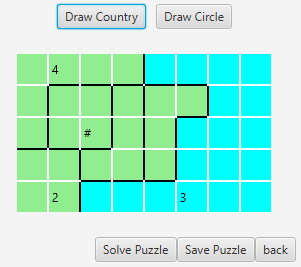
\includegraphics[scale=1]{Pictures/drawing_screen.png} 
  \caption{The drawing screen}
  \label{fig:drawing_screen}
\end{figure}

\subsection{Loading Puzzle} lets one load a saved .pzl-file to play that puzzle.

\chapter{JavaFX} \label{JavaFX}
The GUI was created with JavaFX because of two simple reasons. First it was appealing to keep the whole project in Java to be operating systems independent and secondly JavaFX is rather young and being up to date is important.

\section{What is JavaFX?}
JavaFX was first developed in December 2008 by Oracle Corporation, the current version is JavaFX 8 which was released in May 2014. It is a set of graphics and media packages that enables developers to design, create, test, debug, and deploy client applications that operate consistently across diverse platforms.\footnote{https://docs.oracle.com/javafx/2/overview/jfxpub-overview.htm} 

It was intended to replace Swing as the standard GUI library in Java Standard Edition however both will be included for now. But still JavaFX can be seen a bit as a successor to Swing.

\section{New Features over Swing}
Written as a Java API, JavaFX application code can reference APIs from any Java library. Which means one can use Java API libraries to access native system capabilities. 
Also the web view supports HTML5 and all the goodies that comes with that.

However for this project the most important part is that JavaFX supports Cascading Style Sheets for skinning ones GUI and FXML to define the GUI separately from the application logic.

FXML files are similar to XML files and they contain all the controls of the GUI. In other words one can finally use the Model-View-Controller pattern without violating some of its regulations.

\chapter{Statistics} \label{Statistics}
TODO: requires the tool to be fully done + some time of data-collecting.

\chapter{Conclusion} \label{Conclusion}
TODO: requires the rest of the project to be done.